% style/preamble throws error, hence preamble4tex is kept here
\documentclass[11pt,compress,t,notes=noshow]{beamer}\usepackage[]{graphicx}\usepackage[]{color}

\makeatletter
\def\maxwidth{ %
  \ifdim\Gin@nat@width>\linewidth
    \linewidth
  \else
    \Gin@nat@width
  \fi
}
\makeatother

\definecolor{fgcolor}{rgb}{0.345, 0.345, 0.345}
\newcommand{\hlnum}[1]{\textcolor[rgb]{0.686,0.059,0.569}{#1}}%
\newcommand{\hlstr}[1]{\textcolor[rgb]{0.192,0.494,0.8}{#1}}%
\newcommand{\hlcom}[1]{\textcolor[rgb]{0.678,0.584,0.686}{\textit{#1}}}%
\newcommand{\hlopt}[1]{\textcolor[rgb]{0,0,0}{#1}}%
\newcommand{\hlstd}[1]{\textcolor[rgb]{0.345,0.345,0.345}{#1}}%
\newcommand{\hlkwa}[1]{\textcolor[rgb]{0.161,0.373,0.58}{\textbf{#1}}}%
\newcommand{\hlkwb}[1]{\textcolor[rgb]{0.69,0.353,0.396}{#1}}%
\newcommand{\hlkwc}[1]{\textcolor[rgb]{0.333,0.667,0.333}{#1}}%
\newcommand{\hlkwd}[1]{\textcolor[rgb]{0.737,0.353,0.396}{\textbf{#1}}}%
\let\hlipl\hlkwb

\usepackage{framed}
\makeatletter
\newenvironment{kframe}{%
 \def\at@end@of@kframe{}%
 \ifinner\ifhmode%
  \def\at@end@of@kframe{\end{minipage}}%
  \begin{minipage}{\columnwidth}%
 \fi\fi%
 \def\FrameCommand##1{\hskip\@totalleftmargin \hskip-\fboxsep
 \colorbox{shadecolor}{##1}\hskip-\fboxsep
     \hskip-\linewidth \hskip-\@totalleftmargin \hskip\columnwidth}%
 \MakeFramed {\advance\hsize-\width
   \@totalleftmargin\z@ \linewidth\hsize
   \@setminipage}}%
 {\par\unskip\endMakeFramed%
 \at@end@of@kframe}
\makeatother

\definecolor{shadecolor}{rgb}{.97, .97, .97}
\definecolor{messagecolor}{rgb}{0, 0, 0}
\definecolor{warningcolor}{rgb}{1, 0, 1}
\definecolor{errorcolor}{rgb}{1, 0, 0}
\definecolor{code}{rgb}{0.97, 0.96, 1.0}
\newenvironment{knitrout}{}{} % an empty environment to be redefined in TeX

\usepackage{alltt}
\usepackage[utf8]{inputenc}
\usepackage[ngerman]{babel}
\usepackage{dsfont}
\usepackage{verbatim}
\usepackage{amsmath}
\usepackage{amsfonts}
\usepackage{mathtools}
\usepackage{csquotes}
\usepackage{cmbright}
\usepackage{multirow}
\usepackage{longtable}
\usepackage{enumerate}
\usepackage[absolute,overlay]{textpos}
\usepackage{psfrag}
\usepackage{algorithm}
\usepackage{algpseudocode}
\usepackage{eqnarray}
\usepackage{bytefield}
\usepackage{animate}
\usepackage{tikz}
\usetikzlibrary{shapes,matrix,positioning,chains,arrows,shadows,decorations.pathmorphing,fit,backgrounds}
\usepackage{adjustbox}
\usepackage{colortbl}
\usepackage{tabularx} % for tables (incl. \hline)
\usepackage{arydshln} % Load after array, longtable, colortab and/or colortbl , otherwise problems with \hline in tabular env
\usepackage{etex} %increase registers for \dimenS to more than 256, otherwise we get "No room for a new \dimen"
\usepackage{graphicx}
\usepackage{booktabs} %used in epr lectures
\usepackage{bm} % bold greek letters
\usepackage{hyperref} % url citing
\usepackage{blkarray} % block arrays
\usepackage{listings} % block of code
\usepackage{xcolor} %colored math symbols
\usepackage{pgffor}
\usepackage{verbatimbox}
\usepackage{xcolor}

%some colors
\definecolor{checkgreen}{HTML}{18A126}
\definecolor{errorred}{HTML}{FF0000}
\definecolor{blockbg}{HTML}{F7F7F7}
\definecolor{gray}{HTML}{A0A0A0}

% basic latex stuff
\newcommand{\col}{\par\colorbox{code}{\parbox{\textwidth}{\theverbbox}}\par}
\newcommand{\eg}{e.\,g.\xspace} %for example
\newcommand{\ie}{i.\,e.\xspace} %that is to say...
\newcommand{\pkg}[1]{{\fontseries{b}\selectfont #1}} %fontstyle for R packages
\newcommand{\lz}{\vspace{0.5cm}} %vertical space
\newcommand{\oneliner}[1] % Oneliner for important statements
{\begin{block}{}\begin{center}\begin{Large}#1\end{Large}\end{center}\end{block}}
\def\SpAr{\quad \Rightarrow \quad}

%new environments
\newenvironment{vbframe}  %frame with breaks and verbatim
{
 \begin{frame}[containsverbatim,allowframebreaks]
}
{
\end{frame}
}

\newenvironment{vframe}  %frame with verbatim without breaks (to avoid numbering one slided frames)
{
 \begin{frame}[containsverbatim]
}
{
\end{frame}
}

\newenvironment{blocki}[1]   % itemize block
{
 \begin{block}{#1}\begin{itemize}
}
{
\end{itemize}\end{block}
}

\newenvironment{fragileframe}[2]{  %fragile frame with framebreaks
\begin{frame}[allowframebreaks, fragile, environment = fragileframe]
\frametitle{#1}
#2}
{\end{frame}}

\newcommand{\myframe}[2]{  %short for frame with framebreaks
\begin{frame}[allowframebreaks]
\frametitle{#1}
#2
\end{frame}}

\usepackage{../../style/lmu-lecture}

\let\code=\texttt
\let\proglang=\textsf

\setkeys{Gin}{width=0.9\textwidth}

\usepackage{tikz}
\usetikzlibrary{shapes,arrows,snakes, calc}

% Define block styles
\tikzstyle{decision} = [diamond, draw, text width=6em, text badly centered, node distance=4cm, inner sep=0pt]
\tikzstyle{decision2} = [diamond, draw, fill=customgreen!35, text width=6em, text badly centered, node distance=4cm, inner sep=0pt]

\tikzstyle{block} = [rectangle, draw, text width=14em, text centered, rounded corners, node distance=3cm, minimum height=4em]
\tikzstyle{line} = [draw, -latex']
\tikzstyle{cloud} = [draw, ellipse, node distance=3cm, minimum height=2em]

\title{Introduction to Deep Learning}
\author{Bernd Bischl}
\institute{Department of Statistics -- LMU Munich}
\date{WS 2021/2022}

\setbeamertemplate{frametitle}{\expandafter\uppercase\expandafter\insertframetitle}

\IfFileExists{upquote.sty}{\usepackage{upquote}}{}
\input{../../latex-math/basic-math}
\input{../../latex-math/basic-ml}
\input{../../latex-math/ml-nn}

\newcommand{\titlefigure}{figure/ps11.png}
\newcommand{\learninggoals}{
  \item Sparse Interactions 
  \item Parameter Sharing
  \item Equivariance to Translation
}

\title{Deep Learning}
\date{}

\begin{document}

\lecturechapter{Properties of Convolution}
\lecture{I2DL}
%%%%%%%%%%%%%%%%%%%%%%%%%%%%%%%%%%%%%%%%%%%%%%%%%%%%%%%%%%%%%%%%%%

%%%%%%%%%%%%%%%%%%%%%%%%%%%%%%%%%%%%%%%%%%%%%%%%%%%%%%%%%%%%%%%%%%

\frame{

\frametitle{Sparse interactions}

  \center
  \only<1>{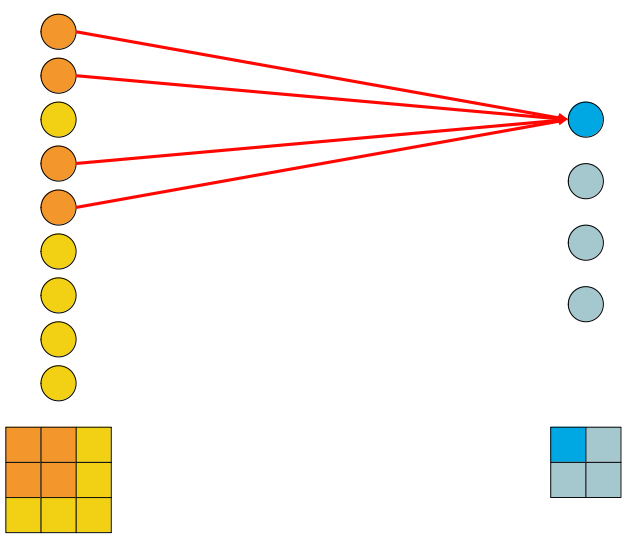
\includegraphics[width=7cm]{figure/sparse1.png}}%
  %\only<2>{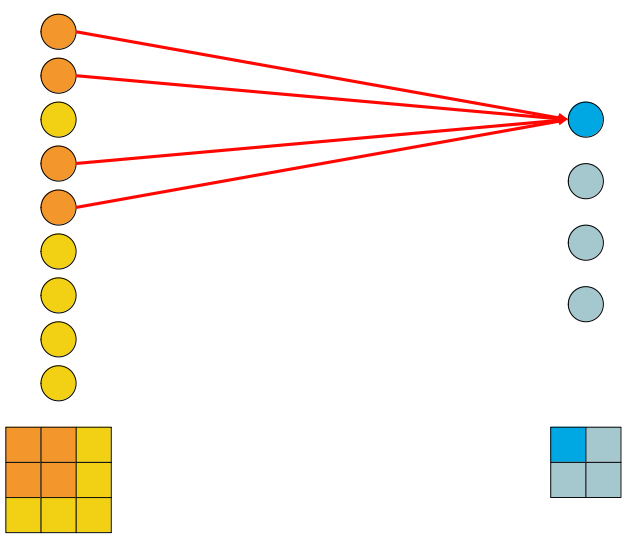
\includegraphics[width=7cm]{figure/sparse1.png}}%
  %\only<3>{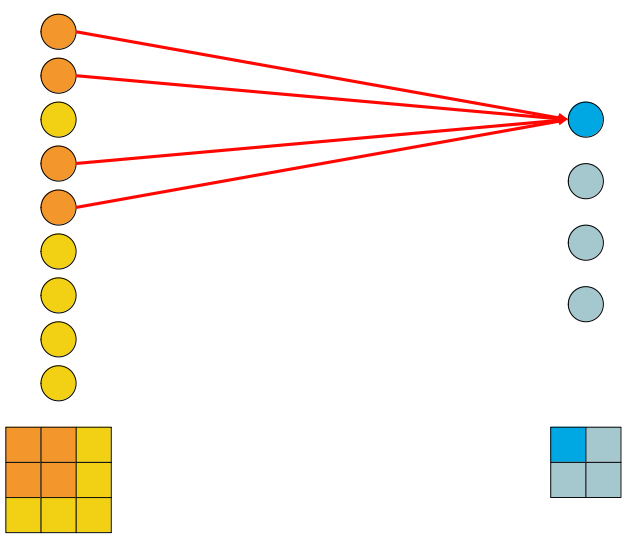
\includegraphics[width=7cm]{figure/sparse1.png}}%
  %\only<4>{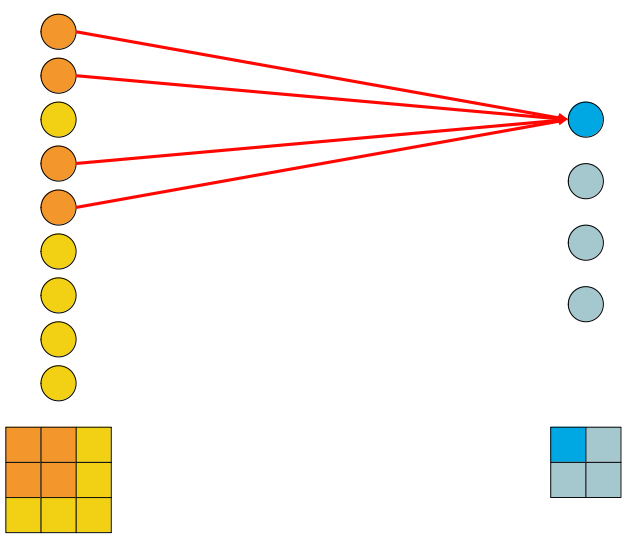
\includegraphics[width=7cm]{figure/sparse1.png}}%
  \only<2>{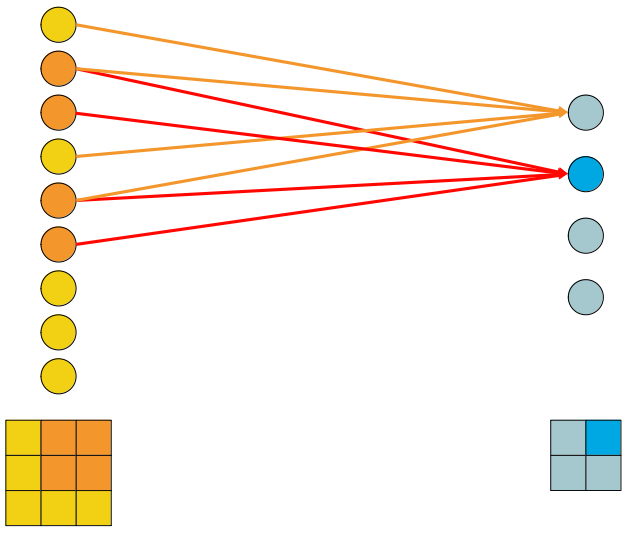
\includegraphics[width=7cm]{figure/sparse2.png}}%
  \only<3>{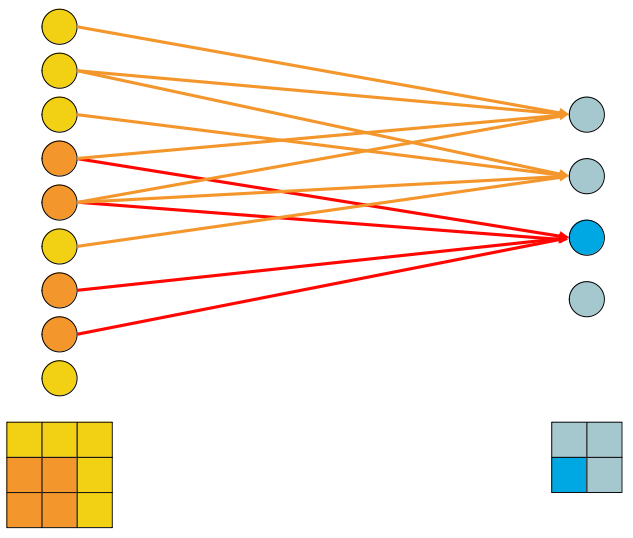
\includegraphics[width=7cm]{figure/sparse4.png}}%
  \only<4>{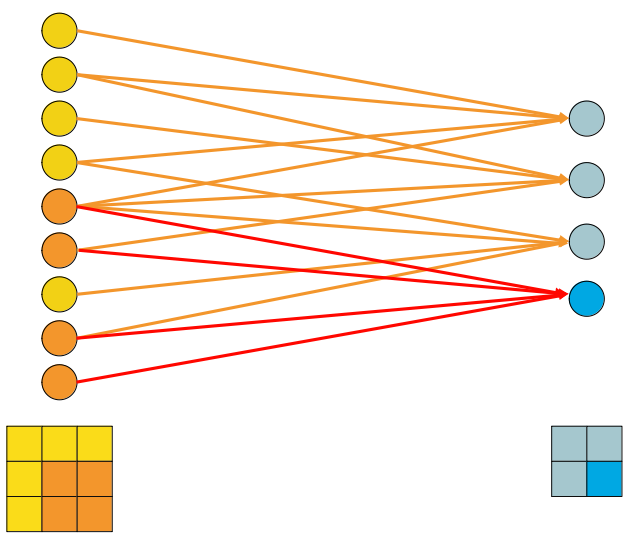
\includegraphics[width=7cm]{figure/sparse5.png}}%
  \only<5>{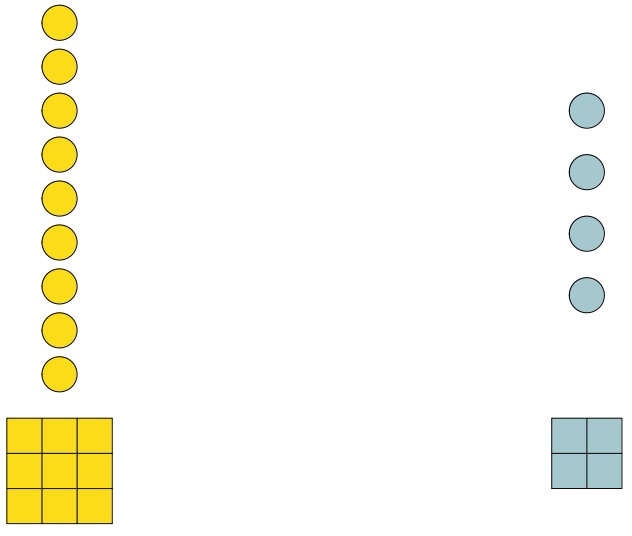
\includegraphics[width=7cm]{figure/sparsedense1.png}}%
  \only<6>{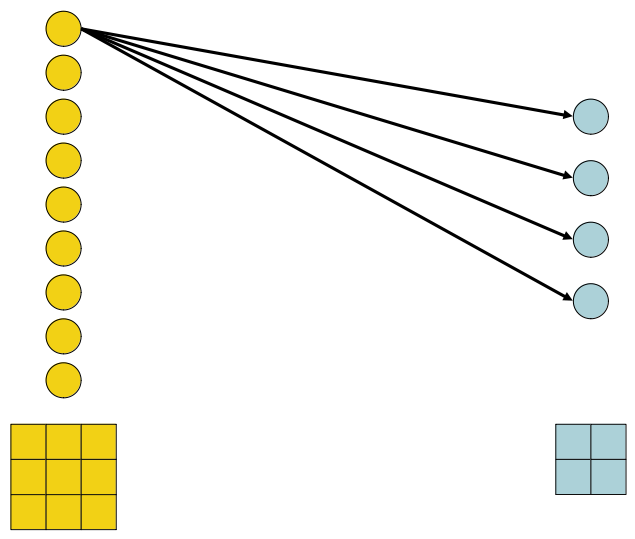
\includegraphics[width=7cm]{figure/sparsedense2.png}}%
  \only<7>{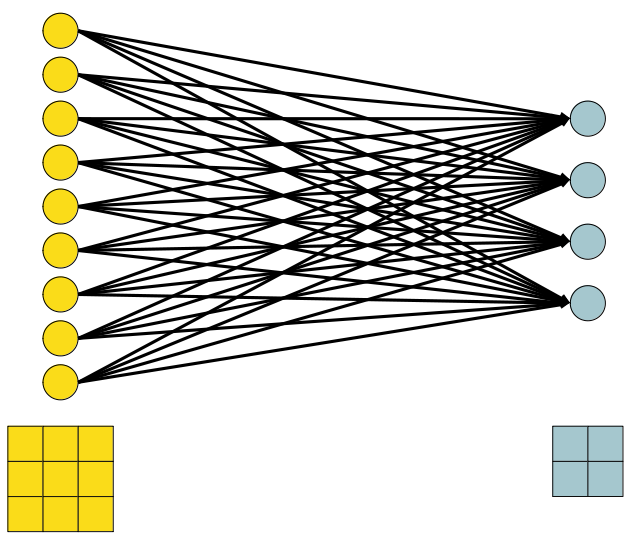
\includegraphics[width=7cm]{figure/sparsedense3.png}}%

  \begin{itemize}

    \only<1>{\item We want to use the \enquote{neuron-wise} representation of our CNN. \item Moving the filter to the first spatial location yields us the first entry of the feature map which is composed of these four connections.}
    %\only<1>{\item Moving the filter to the first spatial location...}
    %\only<1>{\item ...yields us the first entry of the feature map...}
    %\only<4>{\item ...which is composed of these four connections.}
    \only<2>{\item Similarly...}%$s_{12}$ is composed by these four connections.}
    \only<3>{\item Similarly...}%$s_{21}$ by these..}
    \only<4>{\item Similarly...}%{\item and finally $s_{22}$ by these.}
    \only<5>{\item Assume we would replicate the architecture with a dense net.}
    \only<6>{\item Each input neuron is connected with each hidden layer neuron.}
    \only<7>{\item In total, we obtain 36 connections!}

  \end{itemize}

}
%%%%%%%%%%%%%%%%%%%%%%%%%%%%%%%%%%%%%%%%%%%%%%%%%%%%%%%%%%%%%%%%%%
%%%%%%%%%%%%%%%%%%%%%%%%%%%%%%%%%%%%%%%%%%%%%%%%%%%%%%%%%%%%%%%%%%
\begin{frame}{Sparse interactions}
  \begin{itemize}
    \item What does that mean?
    \begin{itemize}
      \item Our CNN has a \textbf{receptive field} of 4 neurons.
      \item That means, we apply a \enquote{local search} for features.
      \item A dense net on the other hand conducts a \enquote{global search}.
      \item The receptive field of the dense net are 9 neurons.
    \end{itemize}
    \item When processing images, it is more likely that features occur at specific locations in the input space.
    \item For example, it is more likely to find the eyes of a human in a certain area, like the face.
    \begin{itemize}
      \item A CNN only incorporates the surrounding area of the filter into its feature extraction process.
      \item The dense architecture on the other hand assumes that every single pixel entry has an influence on the eye, even pixels far away or in the background.
    \end{itemize}
  \end{itemize}
\end{frame}
%%%%%%%%%%%%%%%%%%%%%%%%%%%%%%%%%%%%%%%%%%%%%%%%%%%%%%%%%%%%%%%%%%
%%%%%%%%%%%%%%%%%%%%%%%%%%%%%%%%%%%%%%%%%%%%%%%%%%%%%%%%%%%%%%%%%%

\frame{

\frametitle{Parameter Sharing}

  \center
  \only<1>{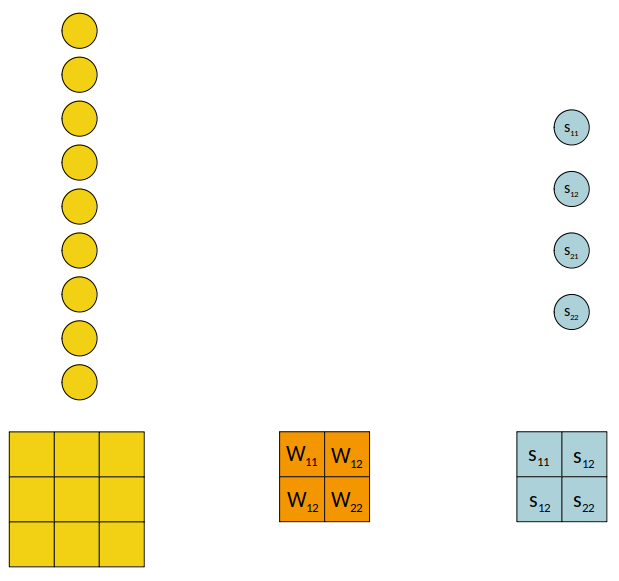
\includegraphics[width=7cm]{figure/ps1.png}}%
  \only<2>{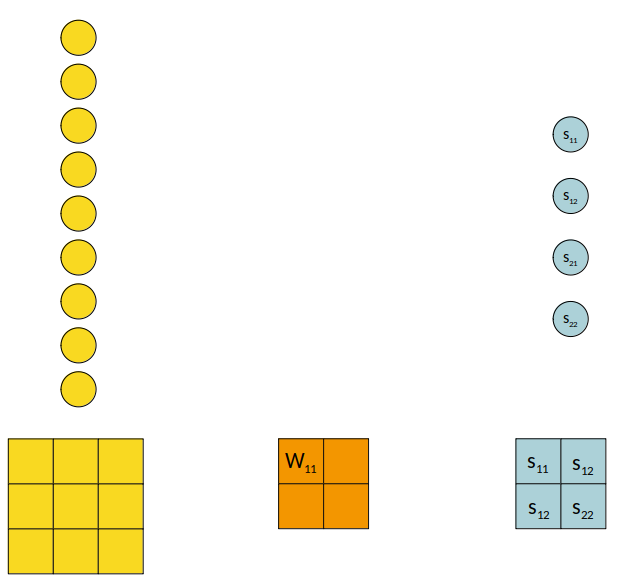
\includegraphics[width=7cm]{figure/ps2.png}}%
  \only<3>{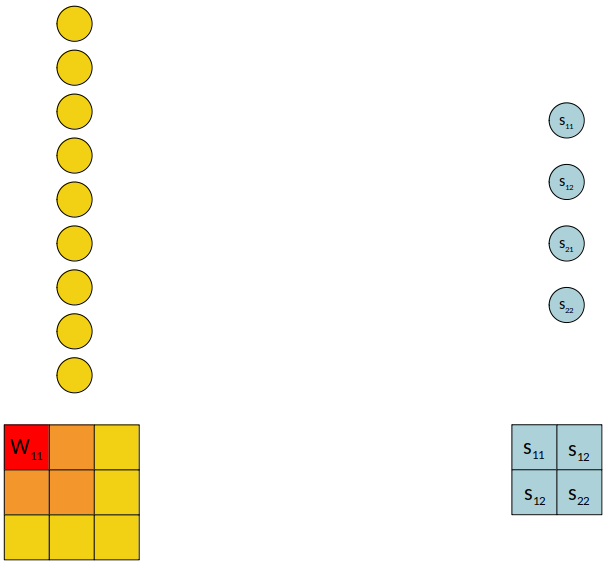
\includegraphics[width=7cm]{figure/ps3.png}}%
  \only<4>{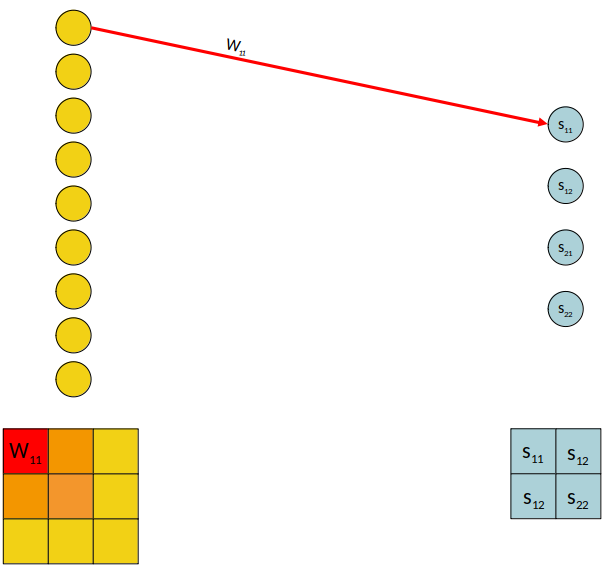
\includegraphics[width=7cm]{figure/ps4.png}}%
  \only<5>{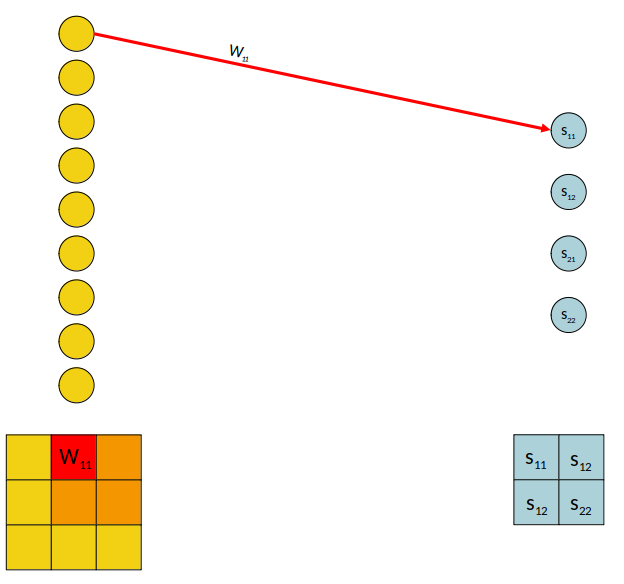
\includegraphics[width=7cm]{figure/ps6.png}}%
  \only<6>{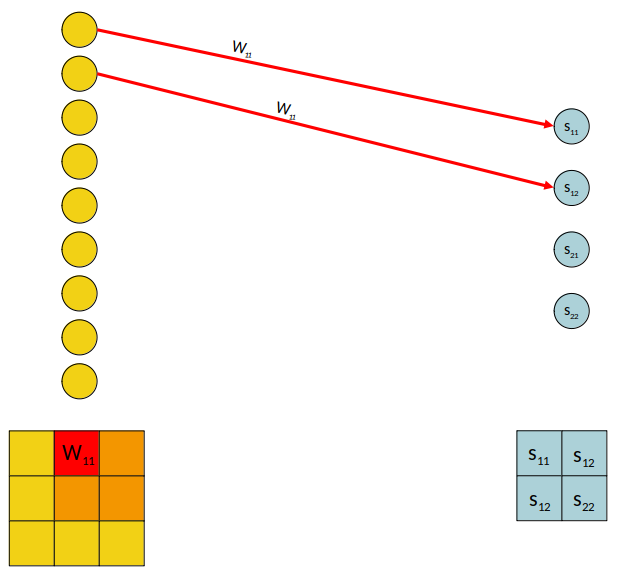
\includegraphics[width=7cm]{figure/ps7.png}}%
  \only<7>{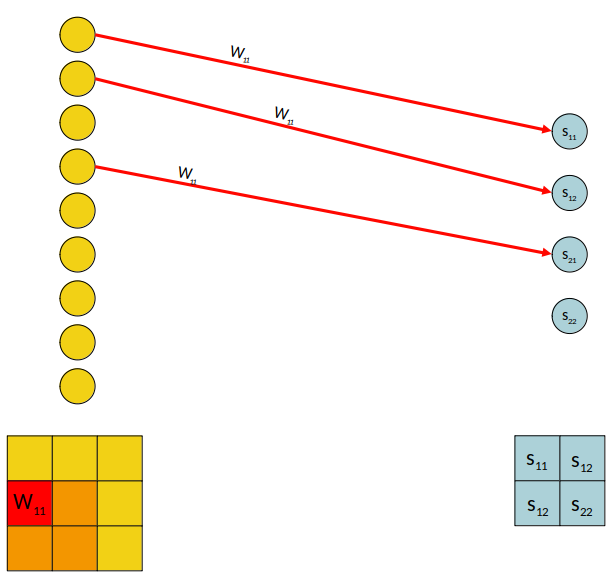
\includegraphics[width=7cm]{figure/ps8.png}}%
  \only<8>{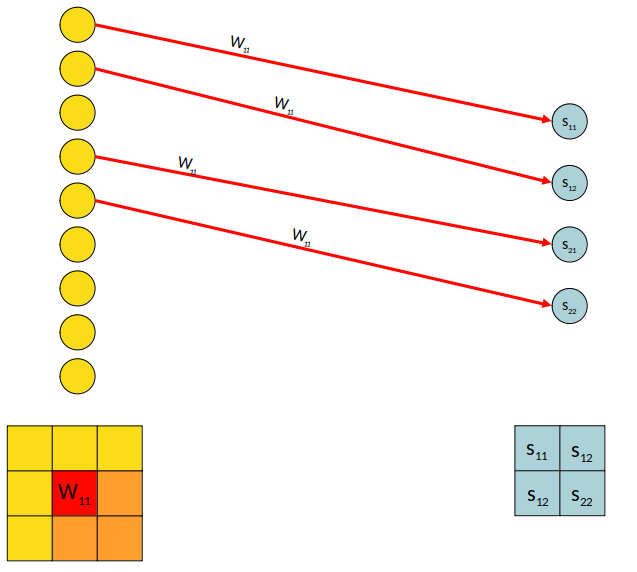
\includegraphics[width=7cm]{figure/ps9.png}}%
  \only<9>{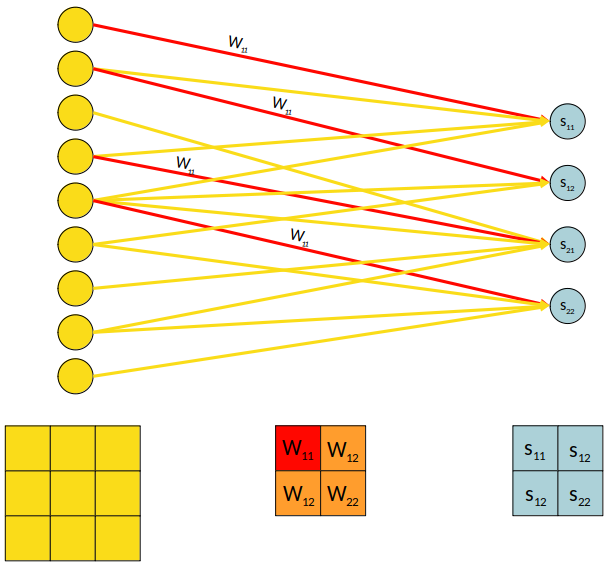
\includegraphics[width=7cm]{figure/ps11.png}}%
  \only<10>{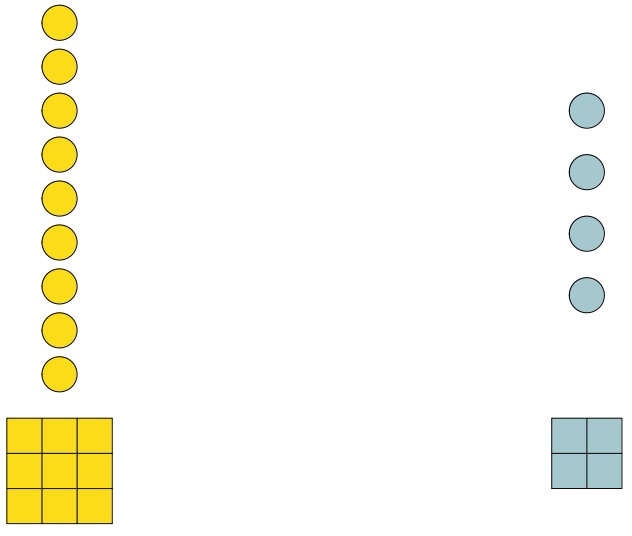
\includegraphics[width=7cm]{figure/sparsedense1.png}}%
  \only<11>{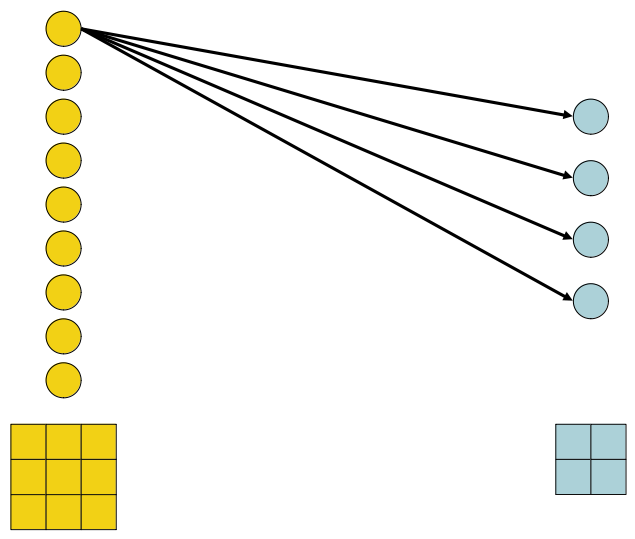
\includegraphics[width=7cm]{figure/sparsedense2.png}}%

  \begin{itemize}

    \only<1>{\item For the next property we focus on the filter entries.}
    \only<2>{\item In particular, we consider weight $w_{11}$}
    \only<3>{\item As we move the filter to the first spatial location..}
    \only<4>{\item ...we observe the following connection for weight $w_{11}$}
    \only<5>{\item Moving to the next location...}
    \only<6>{\item ...highlights that we use the same weight more than once!}
    \only<7>{\item Even three...}
    \only<8>{\item And in total four times.}
    \only<9>{\item All together, we have just used four weights.}
    \only<10>{\item How many weights does a corresponding dense net use?}
    \only<11>{\item $9 \cdot 4 = 36$! That is 9 times more weights!}

  \end{itemize}

}
%%%%%%%%%%%%%%%%%%%%%%%%%%%%%%%%%%%%%%%%%%%%%%%%%%%%%%%%%%%%%%%%%%
%%%%%%%%%%%%%%%%%%%%%%%%%%%%%%%%%%%%%%%%%%%%%%%%%%%%%%%%%%%%%%%%%%
\begin{vbframe}{Sparse Connections and Parameter sharing}
  \begin{itemize}
    \item Why is that good?
    \item Less parameters drastically reduce memory requirements.
    \item Faster runtime:
    \begin{itemize}
      \item For $m$ inputs and $n$ outputs, a fully connected layer requires $m\times n$ parameters and has $\mathcal{O}(m\times n)$ runtime.
      \item A convolutional layer has limited connections $k<<m$, thus only $k\times n$ parameters and $\mathcal{O}(k\times n)$ runtime.
    \end{itemize}
    \item But it gets even better:
    \begin{itemize}
      \item Less parameters mean less overfitting and better generalization!
    \end{itemize}
  \end{itemize}
\framebreak
  \begin{itemize}
    \item Example: consider a color image with size $100 \times 100$.
    \item Suppose we would like to create one single feature map with a \enquote{same padding} (i.e. the hidden layer is of the same size).
    %(i.e. retain the dim of the input for our feature maps).
    \begin{itemize}
      \item Choosing a filter with size $5$ means that we have a total of $5 \cdot 5 \cdot 3 = 75$ parameters (bias unconsidered).
      \item A dense net with the same amount of \enquote{neurons} in the hidden layer results in 
      $$\underbrace{(100^2 \cdot 3)}_{\text{input}} \cdot \underbrace{(100^2)}_{\text{hidden layer}} = 300.000.000 $$ parameters.
      
      %\item A dense net needs $10.000$ neurons in its hidden layer to replicate that architecture ($100 \cdot 100 = 10.000$). It has $100 \cdot 100 \cdot 3 \cdot 10.000 = 300.000.000$ parameters (bias unconsidered)!
      
    \end{itemize}
  \item Note that this was just a fictitious example. In practice we do not try to replicate CNN architectures with dense networks (actually it isn't even possible since physical limitations like the computer hardware would not allow us to).
  \end{itemize}
\end{vbframe}
%%%%%%%%%%%%%%%%%%%%%%%%%%%%%%%%%%%%%%%%%%%%%%%%%%%%%%%%%%%%%%%%%%
%%%%%%%%%%%%%%%%%%%%%%%%%%%%%%%%%%%%%%%%%%%%%%%%%%%%%%%%%%%%%%%%%%

\frame{

\frametitle{Equivariance to translation}

  \center
  \only<1>{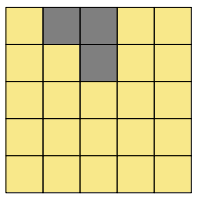
\includegraphics[width=5cm]{figure/equivariance1.png}}%
  \only<2>{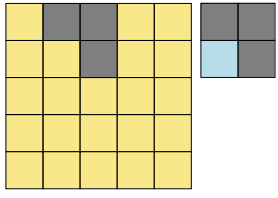
\includegraphics[width=7cm]{figure/equivariance2.png}}%
  \only<3>{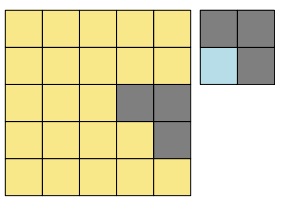
\includegraphics[width=7cm]{figure/equivariance3.png}}%
  \only<4>{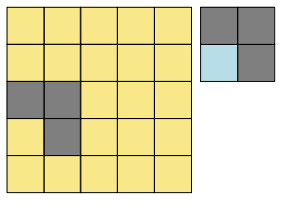
\includegraphics[width=7cm]{figure/equivariance4.png}}%

  \begin{itemize}

    \only<1>{\item Think of a specific feature of interest, here highlighted in grey.}
    \only<2>{\item Furthermore, assume we had a tuned filter looking for exactly that feature.}
    \only<3>{\item The filter does not care at what location the feature of interest is located at.}
    \only<4>{\item It is literally able to find it anywhere! That property is called \textbf{equivariance to translation}. \\[0.2cm] \scriptsize{Note: A function $f(x)$ is equivariant to a function $g$ if $f(g(x)) = g(f(x))$.}}
  \end{itemize}

}

%%%%%%%%%%%%%%%%%%%%%%%%%%%%%%%%%%%%%%%%%%%%%%%%%%%%%%%%%%%%%%%%%%
%%%%%%%%%%%%%%%%%%%%%%%%%%%%%%%%%%%%%%%%%%%%%%%%%%%%%%%%%%%%%%%%%%
\begin{frame}{Nonlinearity in feature maps}
    \begin{itemize}
        \item As in dense nets, we use activation functions on all feature map entries to introduce nonlinearity in the net.
        \item Typically rectified linear units (ReLU) are used in CNNs:
            \begin{itemize}
                \item They reduce the danger of saturating gradients compared to sigmoid activations.
                \item They can lead to \textit{sparse activations}, as neurons $\leq 0$ are squashed to $0$ which increases computational speed.
            \end{itemize}
        \item As seen in the last chapter, many variants of ReLU (Leaky ReLU, ELU, PReLU, etc.) exist.
    \end{itemize}
\end{frame}

%%%%%%%%%%%%%%%%%%%%%%%%%%%%%%%%%%%%%%%%%%%%%%%%%%%%%%%%%%%%%%%%%%

\endlecture
\end{document}
